\chapter{人工智能核心技术}
% 一个总领性的启下段,简单讲一下本章的内容会阐述什么内容

在第三章中,将深入探讨支撑人工智能的核心技术,这些技术是将"人工智能"从理论推向实际应用的关键。人工智能可以被视为一台精密的机器,核心技术则如同机器的引擎,驱动其在现实环境中高效运转并完成多样化任务。

首先聚焦"计算机视觉"这一前沿技术,它赋予机器"看懂"世界的能力,使其能够识别、分析和理解视觉信息。接下来探讨"自然语言智能"技术,这项技术使机器能够理解、处理人类语言,实现人机自然语言交互。最后关注"生成式人工智能"技术,它突破性地赋予机器创造和生成新颖内容的能力,开启了人工智能的新纪元。

通过系统性地剖析这些核心技术,可以清晰地认识到,人工智能并非一个抽象的概念,而是由多项先进技术构成的复杂系统。每一项技术的突破性进展都在推动人工智能在现实世界中发挥日益重要的作用。从智能医疗诊断到自动驾驶系统,从智慧城市管理到个性化推荐服务,人工智能的核心技术不仅正在重塑生活方式,更在不断提升解决复杂问题的能力。

本章将对这些核心技术进行深入剖析,揭示其实现基本任务的技术原理,并展示其在各行业中的创新应用。通过对这些核心技术的全面理解,将更深刻地认识到人工智能如何从基础任务走向实际应用,从理论构想走向现实突破,并在未来持续释放其变革性潜力。

\section{计算机视觉}

计算机视觉作为人工智能的重要分支,致力于赋予计算机“看”的能力,使其能够模拟人类视觉系统进行图像和视频的获取、处理与理解。这一领域融合了图像处理、模式识别、机器学习以及深度学习等多种技术,旨在让机器能够自动识别和解释视觉数据中的复杂信息。计算机视觉的应用广泛且深远,涵盖了从自动驾驶、智能监控到医疗影像分析、增强现实等众多领域。随着算法的不断优化和计算能力的提升,计算机视觉正以惊人的速度发展,推动着各行各业的智能化转型。通过深入研究计算机视觉的核心技术,能够更好地理解其在实现智能化社会中的关键作用及其未来的发展潜力。

\subsection{计算机视觉的奠基者}

在1960年代的一个寒冷冬夜,伦敦的一个实验室里,一位年轻的科学家正对着桌上的计算机显示屏凝视。他的眼前没有闪烁的星光,也没有丰富的自然景象,只有一个充满公式和数据的屏幕。大脑依旧是他的探索目标,但他并不满足于仅仅依赖观察来获取知识,他渴望通过数学的力量揭示视觉如何在大脑中运作。
\begin{figure}[htb]
	\centering
	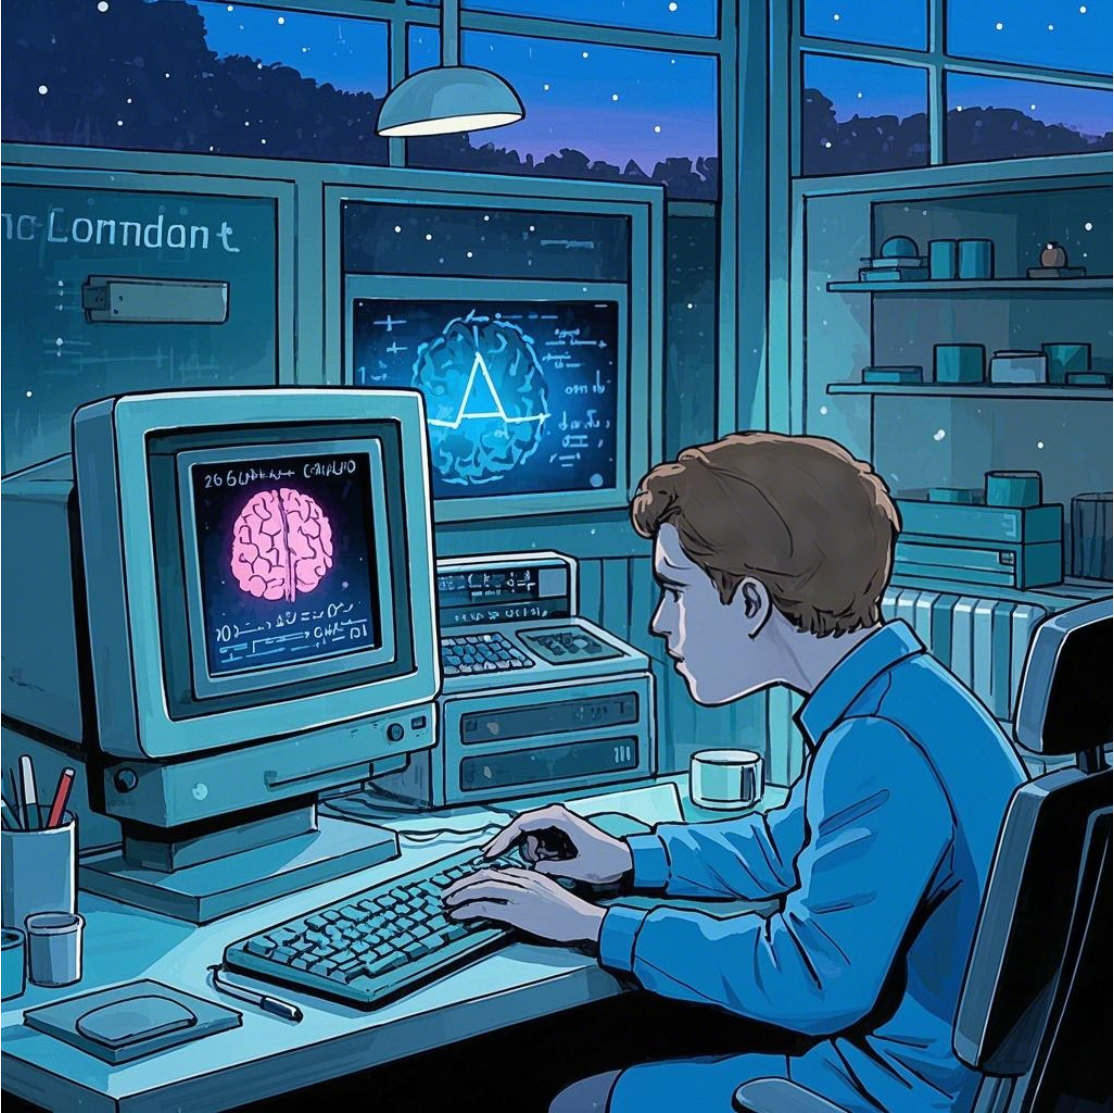
\includegraphics[width=\linewidth]{image/3/3.1.1.png}
\end{figure}

此时他心中疑问着:“我们是如何看见这个世界的?大脑如何从一片光线与阴影中提取出有意义的物体、场景和深度?”他反复思考这个问题,试图从自然界的神经科学研究中找到启示。那时,神经科学家如大卫·休伯尔(David Hubel)\footnote{大卫·休伯尔(1926--2013)是加拿大出生的美国神经生物学家,因其在视觉神经科学方面的开创性研究获得诺贝尔生理学或医学奖。他与托斯滕·维泽尔(Torsten Wiesel)共同研究了视觉皮层的功能,并提出了关于视觉信息处理的分层理论。}和托斯滕·维泽尔(Torsten Wiesel)\footnote{托斯滕·维泽尔(1924--)是瑞典神经生物学家,因其与大卫·休伯尔合作研究大脑视觉皮层的功能,揭示了神经元如何处理视觉刺激而获诺贝尔奖。他们的研究为理解大脑如何处理视觉信息提供了重要线索。}正在研究大脑如何处理视觉信息。他们发现,大脑中的视觉皮层在处理视觉刺激时,特定的神经元负责不同的任务——例如,一些神经元专门识别边缘,有的则专注于深度感知,而其他神经元则负责颜色和运动的处理。这一发现向科学界展示了视觉信息处理的层次性:视觉并非由单一部分进行,而是由多个阶段、不同的区域和不同类型的神经元协同工作。

这一研究启发了年轻科学家的思考:“如果大脑是通过这种分层的方式来处理视觉信息,那么计算机能否也模仿这种结构?”他想,如果计算机能够分阶段、逐步地理解图像,可能就能像人类一样“看见”世界。

于是,他开始构思如何设计一个分层的计算机视觉系统。对于他来说,这不仅是一个科学问题,也是一个哲学性的问题:计算机是否也能像人类一样理解视觉信息?如果可以,它又如何分层理解这些信息?

这位科学家在构建他的视觉系统时,借鉴了当时神经科学和认知科学的最新成果。他逐渐形成了三层次的计算机视觉模型,并将其视为理解“计算机视觉”这一复杂问题的关键:

\begin{itemize}
    \item \textbf{计算理论层次}:首先,他定义了计算机视觉的目标,不仅仅是简单地捕捉图像,更重要的是理解图像中传递的信息,如物体、深度、形状等。他认为,计算机视觉的真正挑战是让计算机理解视觉信息,而不仅仅是处理图像。
    
    \item \textbf{表示与算法层次}:在这个层次,他考虑如何在计算机内部有效地表示这些视觉信息,并设计合适的算法来处理这些信息。每个物体、边缘和线条都需要恰当的数学表示,计算机需要具备识别这些复杂信息结构的能力。只有通过这个层次的处理,计算机才能逐步理解和“看到”图像的结构。
    
    \item \textbf{硬件实现层次}:最后,他考虑如何将这些算法在计算机硬件上实现,这意味着需要设计适当的传感器和硬件来采集和处理视觉信息,使计算机具备“看见”的能力。他提出,计算机视觉不仅仅是算法问题,还涉及感知系统的构建,包括图像输入设备和图像处理硬件。
\end{itemize}

在这个过程中,他不仅受到了神经科学的启发,还受到计算机科学领域几位重要人物的影响。例如,他深入研究了艾伦·图灵(Alan Turing)的计算理论\footnote{艾伦·图灵(Alan Turing,1912--1954)是英国数学家、逻辑学家、密码学家,被誉为计算机科学之父。他提出的“图灵机”模型奠定了计算理论的基础,并为破解第二次世界大战中的德国密码提供了关键帮助。}和约翰·麦卡锡(John McCarthy)的人工智能理论\footnote{约翰·麦卡锡(John McCarthy,1927--2011)是美国计算机科学家,人工智能领域的奠基人之一。他提出了“人工智能”这一术语,并创造了LISP编程语言。McCarthy的研究影响深远,特别是在智能系统和机器学习方面。}。这些理论为他提供了关于如何构建智能系统的深刻启示。他不仅从生物学中借鉴了神经元的分层组织,还借用了计算机科学中的分层思想来构建自己的视觉处理模型。通过结合生物学与计算机科学的知识,他创造了一个全新的计算机视觉框架。

他将这些思考汇总成了自己的著作《视觉》(Vision: A Computational Investigation into the Human Representation and Processing of Visual Information),在书中详细记录了自己如何受到神经科学和早期人工智能领域学者思想的启发。他阐述了一个层次化的视觉处理框架,并提出,计算机视觉不应仅仅视为一个单一的图像处理问题,而应通过多层次的系统逐步解决。从图像的低级特征提取,到更高层次的形状识别、立体视觉,再到最终的对象识别和场景理解,计算机视觉的处理过程应逐步复杂化。

\begin{figure}[htb]
	\centering
	
\includegraphics[width=0.5\linewidth]{image/3/vision.jpg}
\end{figure}


这些想法不仅改变了计算机视觉的研究方向,也为未来的人工智能研究和视觉识别技术的发展提供了新的视角。许多科学家和工程师受到了他的启发,推动了机器视觉、人工智能和计算机视觉技术的发展。通过这些理论,计算机能够更准确地理解视觉信息,推动了自动驾驶、面部识别、图像分类等领域的进步。

这位年轻的科学家就是大卫·马尔(David Marr),他通过将数学、神经科学和计算机科学相结合,揭示了计算机如何“看见”世界的原理。尽管马尔于1980年因病早逝,但他提出的三层次视觉模型成为了计算机视觉的基石,深刻影响了后续的研究与发展。



\begin{figure}[htb]
	\centering
	\includegraphics[width=0.95\linewidth]{image/3/新_David Marr.png}
	\caption{David Marr (图片由 AI 生成)}
\end{figure}

有了三层次的计算机视觉模型作为理论基础,\textbf{计算机图形学}作为人工智能(人工智能)的一个重要组成部分,逐渐发展成为一个独立且不断演进的研究领域。最初,计算机视觉主要集中在简单的图像处理任务上,但随着技术的不断进步,它已经演变为一个涵盖多个方面的复杂学科。如今,计算机视觉的研究不仅仅局限于图像分析,还包括如何使机器“理解”图像和视频内容,并且已广泛应用于各类实际场景。

在计算机视觉的发展过程中,研究者们提出了多种分类方法,以帮助更清晰地理解这一庞大领域。以下是其中一种常见的分类维度\footnote{本节所述的计算机视觉分类维度参考了 ACM Computing Classification System,该系统为计算机科学各领域提供了标准化的分类方法,旨在帮助研究人员和学者更好地理解和讨论不同技术及方法之间的关系。}:

\begin{enumerate}
   \item \textbf{图像与视频采集}  \\
    这部分关注如何从物理世界中采集图像和视频数据。它不仅涉及到\textbf{摄像头}、\textbf{传感器}等硬件设备的设计与优化,还包括如何通过这些设备有效捕捉世界中的动态和静态信息。这是计算机视觉能够“看到”世界的基础。为了实现这些目标,通常需要解决相关的技术问题,如如何提高图像质量、如何减少采集误差等,这些问题与任务密切相关,构成了该子领域的研究内容。

     \item \textbf{计算机视觉表示}  \\
    这部分关注如何表示图像中的结构和特征。可以类比为通过观察人的外貌来判断某些信息。例如,通过一个人的头发颜色、肤色、身高等外貌特征,可以推测他的年龄、职业或个性。这与福尔摩斯通过观察一个人的体态、步伐,甚至是穿着来推断他的职业或性格的方式类似\footnote{福尔摩斯是虚构人物,出现在阿瑟·柯南·道尔的侦探小说中。尽管他并非现实人物,但在这些小说中,他通过细致的观察和推理能够从简单的外貌特征中做出相当了不起的推断。现实中的刑警和侦探也有类似的能力,通过观察和分析案件中的细节特征来推理和解决问题。}。

    在计算机视觉中,计算机通过类似的方式从图像中提取\textbf{特征点}、\textbf{边缘}、\textbf{纹理}等数字信息。正如通过外貌特征可以了解一个人的基本信息,计算机通过这些特征来“理解”图像中的内容。这些数字化的特征为计算机提供了关键线索,帮助其识别图像中的物体、场景,甚至推测图像背后的意义。

 
    \item \textbf{计算机视觉任务}  \\
    计算机视觉任务是指如何让计算机在实际环境中“看见”并理解图像或视频内容。任务更关注“做什么”,即具体应用或功能的目标。任务本身通常是用户或应用系统所需的高层目标。例如,\textbf{物体检测}(找出图像中的物体)、\textbf{图像分类}(把图像归类到不同类别)、\textbf{场景理解}(理解图像中不同元素的关系)等任务,都是通过计算机视觉技术解决的实际问题。而为了完成这些任务,通常需要解决多个相关的技术问题,例如图像分割、目标识别等。这些技术问题构成了完成任务的基础。

    \item \textbf{计算机视觉问题}  \\
    计算机视觉问题更关注“如何做”,即实现任务时需要解决的具体技术或算法难题。例如,\textbf{图像分割}(将图像分成多个有意义的部分)、\textbf{目标识别}(识别图像中的特定对象)、\textbf{跟踪}(追踪移动物体)等问题,都是计算机视觉领域中的关键难题。问题是任务的组成部分,任务本身可以是较高层次的目标,而问题则是实现该目标所需解决的低层次技术难题,仍然是当前研究的重点。
    

\end{enumerate}

(可以通过一个四宫图来简单展示这四个内容)

本节将在后续小节中,通过一些经典的计算机视觉案例,详细阐述相关任务、特征表示、核心问题及技术背后的基本原理与实际应用,以便更深入地理解计算机视觉领域的最新进展及面临的挑战。

\subsection{图像采集与表示}

首先需要了解如何让计算机“看见”世界,即如何通过图像与视频采集设备捕捉图像,并对其进行表示和处理。这是计算机视觉的起点,也是后续让计算机“看懂”和“理解”世界的基础。通过一些问题,可以更好地理解这一过程:

\begin{itemize}
    \item \textbf{问题一:计算机如何捕捉画面?}  

  图像与视频采集技术是计算机视觉的基础,它使得计算机能够通过传感器(如CCD、CMOS摄像头)获取到外部世界的图像和视频数据。通过这些设备,计算机将光线信号转换为电信号,并将其转化为数字图像或视频帧。每个采集设备通过曝光时间、光圈大小、快门速度等参数调整,捕捉到的图像成为计算机进一步处理和理解的原始数据。

    例如,当摄像头捕捉到一个场景时,它通过像素阵列记录下每个位置的光线信息,形成一个图像。每个像素点代表了图像的一部分,它们共同组成了一幅完整的图像。对于视频流来说,这个过程是连续的,每一帧图像就是视频流中的一张静态图像,这些图像帧通过高速捕捉设备被迅速地处理和传输。

    具体来说,假设一个摄像头以每秒30帧的速度捕捉视频,这意味着每秒钟会生成30张静态图像。每张图像由数百万个像素组成,每个像素包含红、绿、蓝(RGB)三个通道的颜色信息。例如,一张分辨率为1920×1080的图像包含约200万个像素,每个像素的RGB值范围在0到255之间,用于表示颜色的深浅和亮度。通过这种方式,摄像头能够精确地记录下场景中的每一个细节。

    在自动驾驶场景中,摄像头捕捉到的实时视频流提供了车辆周围环境的动态画面。例如,一辆自动驾驶汽车可能配备了多个摄像头,分别安装在车头、车尾和两侧。这些摄像头以每秒60帧的速度捕捉视频,每帧图像的分辨率为1280×720。每一帧视频都包括不同物体的位置、形状和颜色信息,计算机可以通过这些信息来实时了解车辆的周围环境。例如,计算机可以通过分析图像中的像素数据,识别出前方的行人、车辆和交通标志,并根据这些信息做出驾驶决策。

    通过这种方式,图像与视频采集技术为计算机视觉提供了丰富的数据源,使得计算机能够“看见”并理解复杂的现实世界。


\item \textbf{问题二:计算机如何理解捕捉到的图像信息?}  

当计算机从摄像头或传感器获取到图像数据后,接下来的问题就是:它如何理解这些图像?对于人类来说,看到一张照片时,人们一眼就能认出其中的物体和场景,比如一只猫、一辆车或一片风景。但对于计算机来说,图像只是一堆数字——每个像素点都有对应的颜色和亮度值,这些数字本身并没有意义。计算机需要通过一系列技术来“读懂”这些数字,从而理解图像的内容。

这个过程可以类比为教一个孩子认识世界。孩子通过观察和反复学习,逐渐学会识别不同的物体。计算机也是如此,它通过“学习”大量的图像数据,慢慢掌握如何从像素中提取有用的信息。具体来说,计算机视觉技术会从图像中提取一些关键特征,比如边缘、颜色、形状等,然后利用这些特征来判断图像中有什么物体。

举个例子,当计算机看到一张猫的照片时,它会先分析图像中的线条和颜色分布,找到猫的轮廓和纹理特征。接着,它会将这些特征与之前“学习”过的猫的图像进行对比,最终判断这张照片中是否有一只猫。这个过程依赖于深度学习技术,尤其是卷积神经网络,它可以帮助计算机从大量数据中学习如何识别物体。

通过这种方式,计算机不仅能“看见”图像,还能“理解”图像中的内容。比如,在自动驾驶中,计算机可以通过分析摄像头拍摄的画面,识别出道路上的车辆、行人和交通标志,从而做出安全的驾驶决策。这种能力让计算机视觉在医疗、安防、娱乐等领域得到了广泛应用。

\item \textbf{问题三:如何应对不清晰的图像?}  

    假设摄像头采集的图像因光线不佳、复杂的环境条件或硬件问题而变得模糊。在这种情况下,计算机如何适应并理解这些不清晰的图像?例如,夜间或恶劣天气下,摄像头可能无法清晰地捕捉到细节,导致图像信息不明确。这种情况类似于人类在视力模糊时通过增强感知或推理来弥补视觉的不足。
w\begin{figure}[htb]
	\centering
	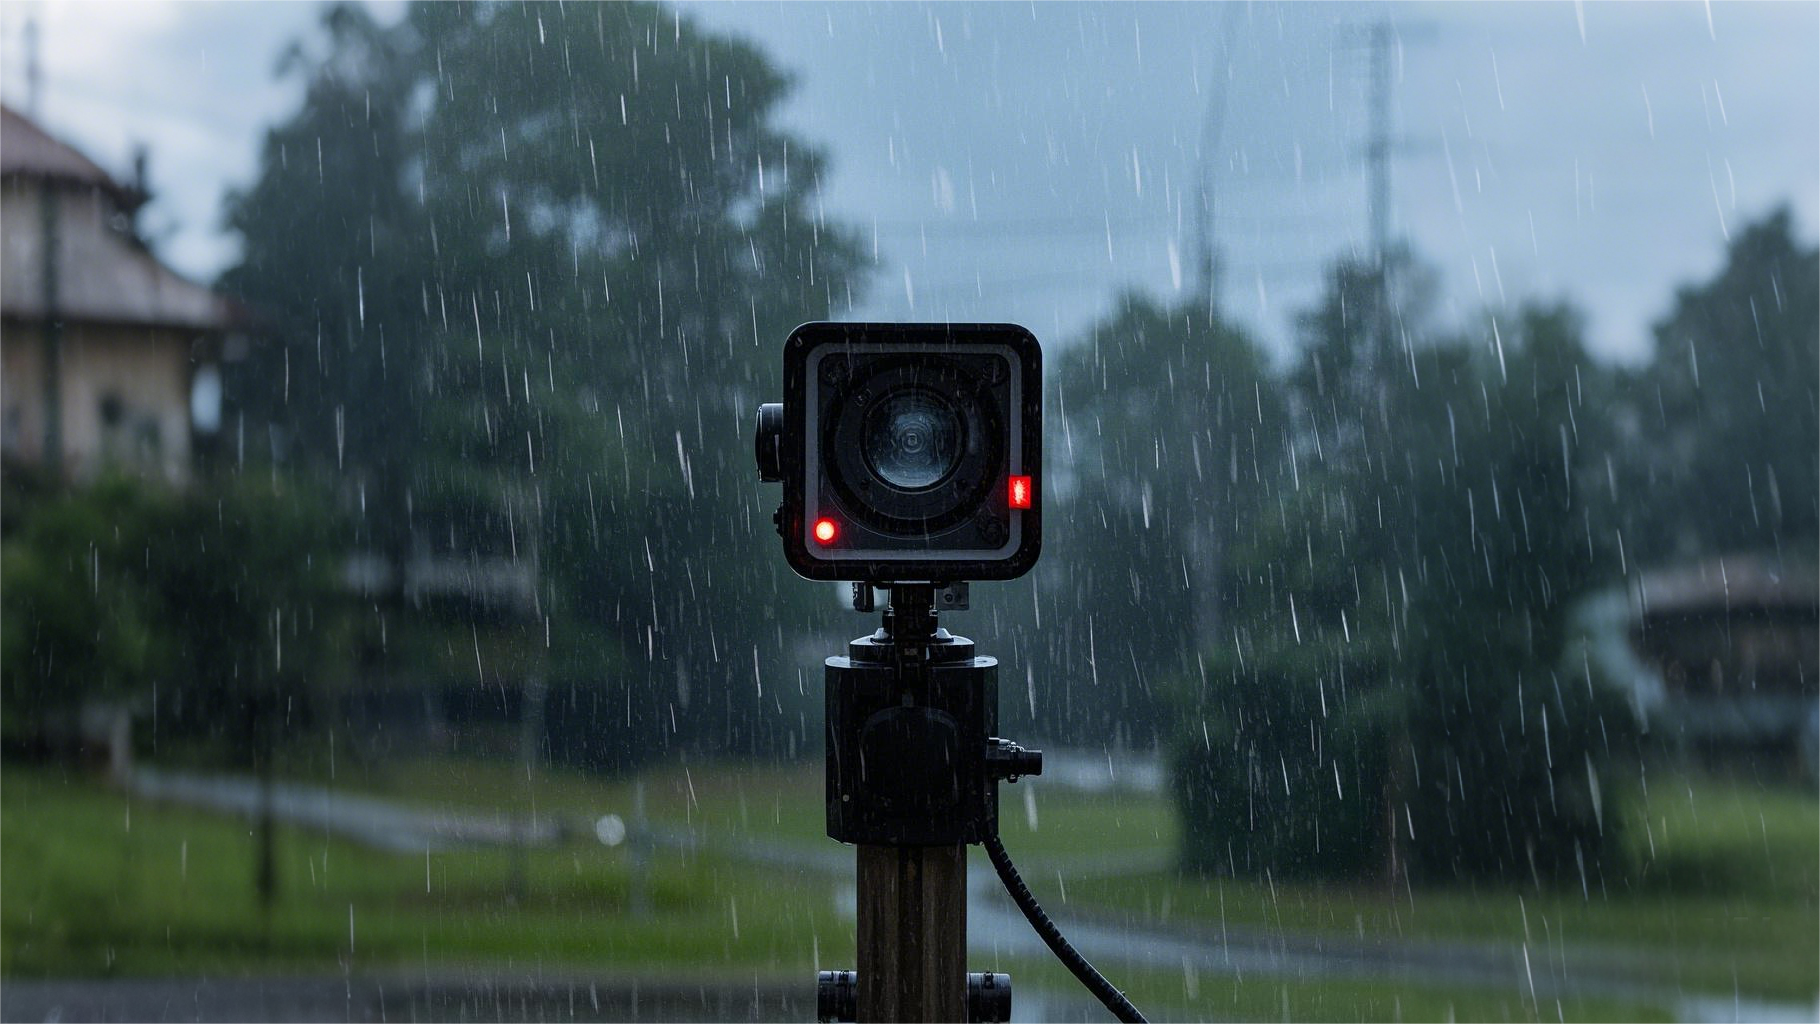
\includegraphics[width=\linewidth]{image/4/暴雨摄像头.png}
	\caption{环境会影响图像的采集质量(图片由 AI 生成)}
\end{figure}
(暴风雨中的摄像头,一张图片)

    对于计算机而言,面对模糊或失真的图像,首先会应用图像增强技术,比如图像去噪、对比度调整等处理手段。具体来说,计算机可能会使用高斯模糊去除噪声,或者通过直方图均衡化来增强图像的对比度。其次,深度学习模型能够在不完美的环境条件下进行推理和补偿,以恢复图像的准确性和可用性。例如,卷积神经网络可以通过训练学习到如何从模糊的图像中提取有用的特征,从而进行准确的识别和分类。此外,生成对抗网络也可以用于图像的超分辨率重建,将低分辨率的图像转换为高分辨率的清晰图像。计算机通过训练和自适应算法,不断提升在复杂环境下的识别能力,从而使其能够在不清晰的图像中做出合理判断。

\end{itemize}

\subsection{计算机视觉任务与问题}

计算机视觉的核心目标是让计算机能够“看见”并理解图像或视频中的内容。为了实现这一目标,计算机视觉领域定义了两类核心内容:任务和问题。任务是实际应用中的高层目标,而问题则是实现这些目标时需要解决的具体技术难题。

\subsubsection{计算机视觉任务:关注“做什么”}

计算机视觉任务关注的是“做什么”,即如何通过技术手段实现具体的功能目标。任务是用户或应用系统所需的高层目标,通常是解决实际问题的最终目的。以下是几个典型的计算机视觉任务:

\paragraph{1. 图像分类}
图像分类是计算机视觉中最基础的任务之一,目标是将图像归类到预定义的类别中。例如,给定一张图片,判断它是猫还是狗。  
\textbf{应用场景:} 图像分类广泛应用于内容管理、医疗影像分析等领域。例如,在医疗影像中,系统可以通过分类任务判断X光片是否显示异常。

\paragraph{2. 物体检测}
物体检测的任务是从图像中找出特定物体的位置,并用边界框标注出来。例如,在一张街景图中检测出行人、车辆和交通标志。  
\textbf{应用场景:} 物体检测是自动驾驶、安防监控等领域的核心技术。自动驾驶车辆需要通过物体检测来识别道路上的行人和其他车辆。

\paragraph{3. 图像分割}
图像分割的任务是将图像分成多个有意义的部分,通常是像素级别的分类。例如,将医学图像中的器官、肿瘤等区域分割出来。  
\textbf{应用场景:} 图像分割在医学影像分析、卫星图像处理等领域有重要应用。例如,医生可以通过分割结果更精确地定位病变区域。

\paragraph{4. 场景理解}
场景理解是更高层次的任务,目标是理解图像中不同元素之间的关系。例如,判断一张图片中的人正在做什么,或者识别出房间内的家具布局。  
\textbf{应用场景:} 场景理解在智能家居、机器人导航等领域有广泛应用。例如,家用机器人可以通过场景理解来识别房间内的物体并执行任务。

\subsubsection{计算机视觉问题:关注“如何做”}

计算机视觉问题关注的是“如何做”,即实现任务时需要解决的具体技术难题。问题是任务的组成部分,通常是低层次的技术挑战,也是当前研究的重点。以下是几个关键的计算机视觉问题:

\paragraph{1. 图像分割}
图像分割是许多任务的基础,但如何将图像准确地分割成有意义的部分仍然是一个难题。例如,在复杂的自然场景中,物体的边界可能模糊不清,导致分割结果不准确。  
\textbf{挑战:} 图像分割需要处理复杂的纹理、光照变化和遮挡问题。近年来,深度学习技术(如全卷积网络FCN)在图像分割中取得了显著进展。

\paragraph{2. 目标识别}
目标识别是物体检测和场景理解的核心问题,目标是识别图像中的特定对象。例如,在一张街景图中识别出行人和车辆。  
\textbf{挑战:} 目标识别需要应对物体的多样性、姿态变化和背景干扰。卷积神经网络和区域建议网络(R-CNN)等技术在目标识别中表现出色。

\paragraph{3. 目标跟踪}
目标跟踪的任务是在视频序列中追踪特定物体的运动轨迹。例如,在监控视频中追踪一个行人。  
\textbf{挑战:} 目标跟踪需要处理物体的外观变化、遮挡和快速运动。近年来,基于深度学习的目标跟踪算法(如SiamFC)在精度和效率上都有显著提升。

\paragraph{4. 图像生成与修复}
图像生成与修复是计算机视觉中的新兴问题,目标是从不完整或低质量的图像中生成高质量的图像。例如,通过生成对抗网络修复模糊的老照片。  
\textbf{挑战:} 图像生成与修复需要处理复杂的纹理和结构信息,同时保持图像的逼真性。GAN和变分自编码器等技术在这一领域取得了重要进展。

\subsubsection{任务与问题的关系}

计算机视觉任务和问题是密不可分的。任务是高层目标,而问题是实现这些目标的技术基础。例如,在自动驾驶中,物体检测是一个任务,而目标识别和图像分割是实现这一任务的关键问题。通过解决这些技术问题,计算机视觉系统能够更好地完成任务,从而在实际应用中发挥作用。

\section{自然语言智能}

是否曾经历过这样的情况:满怀期待地向语音助手发出指令,比如“播放最爱的歌曲”,结果却听到一首完全陌生的曲子,甚至感到失望,恨不得立刻关掉设备?或者在心情愉悦地吩咐“调高温度”时,语音助手却出乎意料地关闭了空调,瞬间置身于寒冷的环境中?更让人抓狂的是,在使用浓重的口音或在嘈杂的环境中尝试与语音助手交流时,所有的努力似乎都化为乌有——它完全无法理解指令。甚至当清晰地说道“打开音乐”时,却放了一段令人不悦的广告。为何会这样?明明这些指令简单而明确,为什么机器总是误解?是否曾幻想过像科幻电影中那样,拥有一个能够像人类一样理解复杂指令并灵活应对的语音助手?然而,现实常常十分无情:系统无法识别指令。显然,计算机在理解人类语言方面仍面临诸多挑战。那么,问题的根源究竟何在?为何对于计算机而言,这样一个看似简单的“语言”任务竟如此复杂?很可能是两个原因:机器听不清,或者机器听不懂。

\subsection{语言识别}

为了深入探讨这一问题,首先需要从语言的复杂性入手。语言,表面上看似是一种直观且易于理解的交流工具,实际上却蕴含着复杂的结构与深刻的含义。语言不仅由单个词汇构成,它的背后隐藏着复杂的语音信号,这些信号受到多种因素的干扰与影响。举例来说,在使用“你好”这一词汇时,不同地区的发音差异即能显现语言的多样性。北京人发出的“你好”与上海人发出的“你好”虽然词汇相同,但由于口音与音调的差异,它们的发音就像两首不和谐的乐曲。即使这两个词汇在书面形式上无异,发音的细微差别使得听者对其产生不同的感知。

此外,环境噪音对语言的影响同样显著。在安静的房间里,语音助手可以轻松地识别用户的指令。然而,当用户处于嘈杂的环境中,例如繁忙的街道,即便大声喊叫,语音助手也可能无法清楚地捕捉到语音信号。这种情形表明,尽管语言是日常生活中频繁使用的工具,计算机仍然面临着“听错”的问题。每一次语言交流都充满了不确定性与多样性,甚至可以将语言的处理比作一场充满挑战的智力游戏,充斥着许多难题与陷阱。

因此,计算机在处理自然语言时,面临的主要挑战是如何从复杂且多变的语音信号中提取出准确的信息。在这一过程中,语音识别技术需要处理发音差异、背景噪音、语音模糊等一系列影响因素,以实现高效而准确的语言理解。先要听清。

\subsubsection{语音识别的基础}

语音识别系统处理复杂信号的过程首先涉及将语言从声音信号中提取出来,简言之,即将声音转化为数字信息。实际上,计算机并非直接“听”到声音,而是将声音信号转化为一系列数字,通过这些数字来理解语音中的信息。该过程通常被称为“声音的数字表示”,并包括两个主要步骤:采样与量化。

采样是将连续的声音信号分割成若干小片段,通常按时间间隔对信号进行采集。每个采样点代表了声音信号在特定时刻的状态。量化则是对声音的振幅进行精确的测量,将连续的振幅值映射为有限数量的离散值,从而使计算机能够处理并理解这些信号。通过这两个步骤,连续的声音信号被转化为一系列数字,供计算机进一步分析和处理。

\subsubsection{采样:声音的“切片”}

可以将声音信号的数字化过程类比为拍摄一张照片。假设正在用相机拍摄一幅风景画,风景是动态的,且不断变化。如果相机不停地拍摄整个景象,它会生成大量的照片,而这些照片代表了风景的各个时刻。

在声音的数字化过程中,采样就像是拍摄这些“瞬间照片”。每次拍摄,相机捕捉到的是某个特定时间点的风景,类似于采样捕捉到的声音信号的振幅。拍摄的频率决定了每秒钟能拍摄多少张照片,这就是采样频率。拍得越频繁,照片中包含的细节就越多。如果相机每秒拍摄1000次(即1000张照片),人们就能捕捉到风景的更多细节。但是,如果拍得太频繁,照片数量太多,就可能导致处理这些照片的时间过长,甚至会占用过多的存储空间,影响效率。

同样的道理,采样频率过低,可能会漏掉一些重要的细节,导致图像不完整,声音失真;而采样频率过高,虽然能捕捉到更多细节,却会带来更大的计算和存储负担。因此,选择合适的采样频率,类似于选择相机的拍摄频率,是为了在捕捉细节和保持效率之间找到平衡。
\begin{figure}[htb]
	\centering
	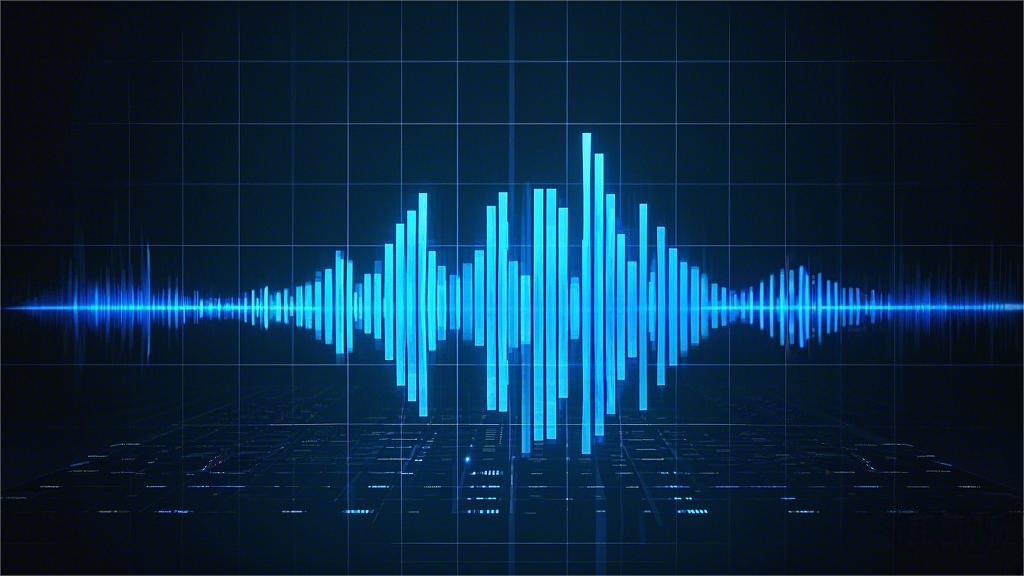
\includegraphics[width=\linewidth]{image/4/音波.png}
	\caption{音波(图片由 AI 生成)}
\end{figure}
而量化过程就像是对这些照片进行编辑。拍摄得到的照片通常是彩色的,每个像素有不同的色彩和亮度。量化就像是给每个像素分配一个固定的颜色等级,可能只有几个不同的选项。量化的精度决定了颜色等级的数量,也决定了照片的细腻程度。颜色等级越多,照片看起来越真实,但处理这些照片的计算量也越大;如果颜色等级太少,照片的色彩就会失真,像素的细节也不清晰。量化精度需要在图像质量和处理负载之间做出权衡。

\subsubsection{量化:音量的“像素化”}

为了帮助理解量化过程,可以借用“像素格子”的类比。设想一张数字化的图片,画面由无数小格子(像素)组成。每个像素呈现一定的颜色和亮度,这些像素的组合共同构成整张图片。提高屏幕的分辨率时,图片中的像素数增多,细节更加丰富;反之,分辨率低时,画面中的像素较少,细节变得模糊。

量化在声音处理中起着类似“像素化”的作用。当计算机处理声音信号时,首先通过采样将声音信号切分成若干个片段,每个片段代表一个时间点的声音振幅。接下来,量化过程将这些振幅映射到一个有限的数值范围,就像给每个声音片段分配一个“像素值”。

例如,8-bit量化将振幅值分为256个等级,16-bit量化将振幅分为65536个等级。每个等级相当于图片中的一个像素,决定了声音细节的呈现精度。如果量化精度较低,相当于低分辨率,声音细节会丢失,呈现出“粗糙”的效果;如果量化精度过高,相当于高分辨率,虽然能够更精确地表达声音细节,但处理和存储的负担也会增大。

就像在低分辨率的图片中,图像细节会被“模糊”掉,声音量化精度低时,细微的音量变化也会被忽略,导致音频失真。然而,过高的量化精度类似于过高分辨率的图像,可能会造成系统处理更多数据,从而浪费存储空间并增加计算负担。

因此,量化的关键在于选择合适的精度,使声音的数字表示尽量精确,同时避免带来过大的计算负担。这个精度的选择类似于在数字图像处理中决定使用多少“像素”来表示画面细节——既要保证图像的清晰度,又要平衡处理效率。

\subsubsection{采样与量化的博弈}

在语音识别中,采样和量化是两个至关重要的过程,它们共同决定了声音信号如何被转换为计算机能够处理的数字格式。采样是将声音信号在时间维度上离散化,而量化则是在幅度维度上对这些离散信号进行离散化,使其能够以数字信号的形式进行处理。

过低的采样率或不足的量化精度会导致声音信号的失真,这就如同通过模糊的画面去判断披萨的味道,无法准确还原真实的声音。而过高的采样率和量化精度,虽然可以提供更为精细的声音细节,却会增加计算资源的消耗,导致效率低下,犹如将披萨切割得过于细碎。

因此,采样与量化之间需要找到一个平衡点,既能高效地捕捉声音的关键特征,又不至于使系统承受过重的计算负担。这一平衡点是在速度与准确性之间的妥协,也是语音识别技术持续研究的重点。

在采样方面,低比特率语音编码技术如混合激励线性预测编码(MELP, Mixed Excitation Linear Prediction)和增强语音服务(EVS, Enhanced Voice Services)通过降低传输带宽需求,确保语音质量,成为语音识别领域的重要研究方向。例如,艾伦·麦克克里(Alan McCree)\footnote{艾伦·麦克克里(Alan McCree)是语音编码领域的知名学者,他开发的MELP编码器在低比特率语音通信中具有重要应用。}开发的MELP编码器已经被广泛应用于低比特率语音通信,并成为北约的标准。

在量化方面,杰弗里·辛顿(Geoffrey Hinton)\footnote{杰弗里·辛顿(Geoffrey Hinton)是深度学习领域的先驱,被誉为“深度学习之父”,他在神经网络和人工智能领域做出了开创性贡献。}和邓力(Li Deng)\footnote{邓力(Li Deng)是语音识别和深度学习领域的专家,曾任微软首席人工智能科学家,在语音识别和自然语言处理方面有重要研究成果。}将深度神经网络引入语音识别,显著提高了量化精度与系统性能。尽管这些技术取得了显著进展,但依然面临语言多样性和复杂环境因素的挑战,如口音和噪声问题。当前的研究方向包括基于神经网络的语音增强技术,以提高系统的鲁棒性。

这一系列突破离不开深度神经网络在语音识别中的应用。深度神经网络不仅改变了量化方式,还重新定义了语音识别的整体框架,使得语音识别从传统的基于规则的方法转向数据驱动的智能化模式。接下来,将重点探讨深度神经网络如何在语音识别领域带来革命性的变化。


\subsubsection{深度识别技术带来的突破}


在语音识别技术的发展过程中,传统的语音识别方法和深度学习驱动的语音识别方法在适应复杂语言特征和环境噪声方面表现出了显著的差异。传统语音识别方法通常依赖于手工设计的规则和模型,而深度神经网络则通过大规模数据训练和自动特征学习,推动了语音识别技术的革命。

\subsubsection{传统语音识别模型}

传统的语音识别系统通过将音频信号转换为数字特征,然后与预先构建的词库和发音模板进行比对,从而实现语音识别。然而,这种方法存在显著的局限性,主要依赖于大量人工设计的规则和模板。这些规则在应对口音差异、语速变化以及背景噪声等复杂的语言特征和环境因素时,往往表现不佳,难以实现高准确率和鲁棒性。因此,传统语音识别系统在多样化和动态变化的实际应用场景中,面临着适应性不足的挑战。

\begin{itemize}
    \item \textbf{口音与方言的适应性差}:传统方法依赖于词库中预定义的发音模板,这些模板通常是基于标准发音训练的,对于不同地区、不同语言环境下的口音和方言,系统难以做出准确的识别。例如,北京口音和上海口音的发音差异会使得传统系统难以准确识别“吃饭”这一词汇。
    \item \textbf{对噪声的鲁棒性较差}:传统系统在处理嘈杂环境下的语音信号时,常常容易受到背景噪声的干扰,导致识别准确性大大降低。例如,在街头或有多人交谈的房间,传统系统很容易将噪音误识别为语音信号,影响识别效果。
    \item \textbf{对语速变化的适应性弱}:传统方法在处理语速加快或变化较大的语音时,也容易出现识别错误。这是因为这些系统通常依赖于静态的发音模型,而不能灵活应对语速的变化。
\end{itemize}

\subsubsection{深度语音识别模型}

深度神经网络对语音识别领域的贡献是革命性的,它使得语音识别技术从传统的规则驱动方法转向了基于数据驱动的学习方法。深度神经网络通过模拟人类大脑的神经网络结构,自动从大规模语音数据中提取音频特征,并逐层构建对语言的理解。这种方式使得深度神经网络能够在复杂的语言特征和环境噪声中表现出色。

\begin{itemize}
    \item \textbf{口音和方言的适应性强}:深度神经网络通过大规模语音数据的训练,能够自动识别和适应不同口音和方言的发音差异。传统方法需要人工构建不同口音的发音模板,而深度神经网络可以通过学习不同口音的共性特征,自动调整其识别策略,从而提高对不同地区语言的识别准确性。例如,当上海话口音的“hello”被说出来时,深度神经网络能够根据学习到的口音特征正确识别出该词汇。
    \item \textbf{提高噪声鲁棒性}:深度神经网络能够从包含噪声的语音数据中学习有用的特征,从而忽略背景噪声的干扰。例如,在嘈杂的街头环境中,深度神经网络可以准确识别出“我要买票”这一语音信号,即便周围有大量的车流和人群噪音。与传统模型相比,深度神经网络在噪声环境中的表现要更为稳健。
    \item \textbf{应对语速变化的能力}:深度神经网络通过多层次的特征提取,能够自动适应语速的变化。它能够通过上下文信息推测出语句的意义,而不需要依赖固定的发音规则。例如,深度神经网络可以在语速较快时仍然准确地识别语音中的每个单词,避免因语速过快而导致的识别错误。
    \item \textbf{上下文感知能力}:深度神经网络不仅能识别单个词汇,还能根据上下文推断出词汇的实际含义。这种上下文感知能力帮助深度神经网络在面对同音词和语义相近的词汇时,能够根据句子的整体意思来做出正确的判断。例如,在“我去买菜”这一句子中,深度神经网络不仅能识别出单个词汇,还能通过上下文推断出每个词汇的语义,从而提高了语句的理解准确性。
\end{itemize}

\subsubsection{}

尽管传统语音识别模型在某些应用场景下仍然有一定的优势,但其局限性在面对复杂的口音、方言、噪声以及语速变化时显得尤为明显。深度神经网络的引入,不仅克服了这些问题,还大大提高了语音识别的准确性和鲁棒性。通过大规模数据的训练和自动特征学习,深度神经网络能够有效地应对不同的语言变化和环境噪声,进而推动了语音识别技术的革命。

然而,尽管深度神经网络在语音识别方面取得了显著进展,仍然面临着一些挑战,如极端噪声环境和复杂语言情境下的表现问题。随着更多创新技术的引入,语音识别技术将变得越来越智能,能够处理更加复杂和多样的语言识别任务。
\footnote{
对于想要深入了解深度学习原理及其在语音识别中的应用的读者,可以参考以下资料:
\begin{itemize}
\item \textit{《深度学习》}(Ian Goodfellow, Yoshua Bengio, Aaron Courville) — 深度学习的权威教材,涵盖神经网络的基础和应用。
\item \textit{《语音与语言处理》}(Daniel Jurafsky \& James H. Martin) — 一本全面讲解语音识别与自然语言处理的书籍,适合对语音识别原理有深入兴趣的读者。
\end{itemize}
}


\subsection{自然语言处理}

自然语言处理(NLP, Natural Language Processing)技术是实现人机语音交流的最后一步关键。在前面的步骤中,语音识别技术让机器“听清”了人类的语音并将其转换为文本;而到了自然语言处理这一步,机器需要进一步“听懂”这些文本的含义,并生成合适的响应或执行相应的操作。NLP 结合了语言学、计算机科学和机器学习的技术,广泛应用于文本分析、语音识别、机器翻译、对话系统等领域。随着深度学习和大数据技术的发展,NLP 的能力得到了显著提升,能够处理更加复杂和多样化的语言任务。

\subsubsection{内容识别}



在日常生活中,文本无处不在——从社交媒体上的推文、新闻文章,到电子邮件、书籍和网页内容。这些文本中蕴含着大量的信息,但对于计算机来说,理解这些信息并不像人类那样直观。这就是内容识别技术的用武之地。内容识别是自然语言处理(NLP)中的一项核心技术,它的目标是让计算机能够从文本中提取有意义的信息,并理解文本的主题、结构以及其中包含的关键元素。简单来说,内容识别就是让计算机“读懂”文本。它不仅仅是简单地识别文本中的单词,而是通过分析文本的语义、结构和上下文,提取出有用的信息。例如,计算机可以从一段新闻文章中识别出主要人物、事件发生的时间和地点,甚至理解文章的主题是体育、科技还是政治。内容识别的核心任务包括分词、词性标注、命名实体识别(NER)和语义分析。通过这些技术,内容识别能够帮助计算机从海量文本中提取出关键信息,为后续的分析和应用提供基础。

内容识别技术的应用非常广泛,几乎涵盖了所有需要处理文本的领域。当使用搜索引擎时,输入一个关键词后,搜索引擎会迅速返回相关的网页或文档。这背后就离不开内容识别技术。搜索引擎会分析输入的查询内容,理解搜索意图,并从海量的网页中筛选出最相关的结果。例如,如果搜索“2023年诺贝尔奖得主”,搜索引擎会识别出“2023年”是时间,“诺贝尔奖”是事件,“得主”是关键词,然后返回相关的新闻报道或百科页面。新闻网站每天都会发布大量的文章,内容涵盖体育、科技、财经、娱乐等多个领域。内容识别技术可以自动将这些文章归类到不同的主题中。例如,一篇关于世界杯的报道会被归类到“体育”类别,而一篇关于人工智能的新闻则会被归类到“科技”类别。这种自动分类不仅方便用户浏览,还能帮助新闻平台更好地组织和管理内容。在某些专业领域,如医学、法律或金融,从大量文本中提取特定信息是非常重要的。例如,医学研究人员可能需要从成千上万的医学文献中提取出某种药物的名称及其疗效;律师可能需要从法律文件中提取出关键条款或判例。内容识别技术可以自动化这一过程,大大节省时间和人力成本。许多公司使用智能客服系统来处理用户的咨询。内容识别技术可以帮助系统理解用户的问题,并从知识库中找到相关的答案。例如,如果用户问“如何重置密码?”,系统会识别出“重置密码”是关键词,并返回相关的操作指南。在社交媒体上,用户每天都会发布大量的文本内容,如推文、评论和帖子。内容识别技术可以分析这些内容,提取出用户讨论的热点话题、情感倾向以及关键人物或事件。例如,品牌可以通过分析社交媒体上的用户评论,了解消费者对某款产品的评价。

内容识别的实现依赖于多种自然语言处理技术。分词是内容识别的第一步。对于英语等以空格分隔单词的语言来说,分词相对简单;但对于中文、日文等没有明显分隔符的语言,分词则是一个复杂的任务。例如,句子“我爱自然语言处理”需要被分割为“我/爱/自然语言/处理”。词性标注是指为每个词语标注其词性,如名词、动词、形容词等。例如,在句子“苹果是一种水果”中,“苹果”被标注为名词,“是”被标注为动词。命名实体识别是指识别文本中具有特定意义的实体,如人名、地名、日期、组织等。例如,在句子“比尔·盖茨是微软的创始人”中,“比尔·盖茨”被识别为人名,“微软”被识别为组织。语义分析是内容识别中最复杂的部分,它旨在理解文本的含义和上下文关系。例如,句子“他打开了窗户,因为房间里很热”中,语义分析需要理解“打开窗户”和“房间里很热”之间的因果关系。

近年来,深度学习技术的快速发展极大地推动了内容识别技术的进步。传统的自然语言处理方法主要依赖于规则和统计模型,而深度学习则通过神经网络模型自动学习文本的特征和规律。BERT(Bidirectional Encoder Representations from Transformers)是一种基于 Transformer 的深度学习模型,它能够同时考虑文本的上下文信息。例如,在句子“他去了银行存钱”中,BERT 能够理解“银行”指的是金融机构,而不是河岸。GPT(Generative Pre-trained Transformer)是一种生成式预训练模型,它不仅可以理解文本,还能生成高质量的文本。GPT 在内容识别中的应用包括文本摘要、问答系统等。这些深度学习模型在内容识别任务中表现出色,能够更准确地理解文本的语义和上下文关系,从而提高了内容识别的效果。

随着人工智能技术的不断发展,内容识别的能力将越来越强大。未来,内容识别技术可能会在多语言支持、跨模态理解和实时处理等方面取得突破。多语言支持将使内容识别技术能够处理更多语言,尤其是低资源语言;跨模态理解将结合文本、图像、音频等多种模态的信息,实现更全面的内容理解;实时处理则将在直播、会议记录等场景中实现高效的内容识别。总之,内容识别技术正在改变人们与文本交互的方式,让计算机能够更好地理解和利用语言数据。无论是搜索引擎、新闻分类,还是智能客服和信息提取,内容识别都在为生活和工作带来便利。随着技术的不断进步,它的应用场景将会更加广泛,成为推动智能化社会发展的关键力量。


\subsubsection{情感识别}

在当今信息爆炸的时代,文字不仅是传递信息的工具,更是表达情感的重要载体。无论是社交媒体上的评论、新闻文章中的观点,还是客户反馈中的评价,文字背后往往蕴含着丰富的情感信息。然而,对于计算机来说,理解这些情感并不像人类那样直观。这就是情感识别技术的意义所在。情感识别,也称为情感分析(Sentiment Analysis),是自然语言处理(NLP)中的一个重要研究方向,旨在分析文本中表达的情感倾向。它可以帮助计算机判断一段文本是正面的、负面的还是中性的,甚至可以识别更复杂的情感状态,如愤怒、喜悦、悲伤等。通过情感识别,计算机能够从海量文本中提取出情感信息,为各行各业提供有价值的洞察。

情感识别技术的应用场景非常广泛,几乎覆盖了所有需要理解人类情感的领域。在社交媒体上,用户每天都会发布大量的评论、帖子和推文,这些内容中蕴含着公众对某一事件、产品或品牌的态度。通过情感识别技术,企业可以分析这些内容,了解消费者对某款产品的评价是正面还是负面,从而调整营销策略或改进产品设计。例如,一家手机制造商可以通过分析社交媒体上关于新机型的评论,发现用户对电池续航时间的抱怨,进而优化下一代产品的设计。在客户服务领域,情感识别技术可以帮助企业分析客户反馈,了解客户对产品或服务的满意度。例如,电商平台可以通过分析用户的评价,识别出哪些商品受到了高度赞扬,哪些商品存在质量问题。这种分析不仅可以帮助企业改进服务,还能为消费者提供更精准的推荐。此外,情感识别技术还可以用于市场趋势预测。通过分析新闻、博客或论坛中的情感倾向,企业可以预测市场情绪的变化趋势。例如,如果某款新技术的相关报道普遍呈现积极情感,那么这项技术可能会在未来成为市场热点;反之,如果某类产品的负面评论增多,则可能预示着市场需求的下降。

情感识别的实现依赖于多种自然语言处理技术和机器学习算法。传统的情感识别方法主要基于规则或统计模型,使用情感词典来判断文本的情感倾向。情感词典是一种包含大量词语及其情感极性(正面、负面或中性)的数据库。例如,词语“优秀”可能被标注为正面情感,而“糟糕”则被标注为负面情感。通过统计文本中正面和负面词语的数量,系统可以判断文本的整体情感倾向。然而,这种方法存在一定的局限性,因为它无法很好地处理上下文信息和复杂的情感表达。例如,句子“这部电影并不糟糕”虽然包含负面词语“糟糕”,但整体表达的情感却是正面的。为了解决这些问题,现代的情感识别方法更多地采用深度学习模型,如长短期记忆网络(LSTM)和 Transformer。这些模型能够捕捉文本中的语义和上下文信息,从而更准确地识别情感倾向。例如,基于 Transformer 的 BERT 模型可以通过双向编码器同时考虑文本的前后文信息,从而更准确地理解句子的情感含义。

情感识别技术的发展不仅依赖于算法的进步,还需要大量的标注数据来训练模型。标注数据是指人工标注了情感极性的文本数据,例如“这家餐厅的服务非常好”被标注为正面情感,“航班延误让我非常失望”被标注为负面情感。通过使用这些标注数据,机器学习模型可以学习如何从文本中提取情感特征,并在新的文本上进行情感预测。近年来,随着社交媒体和在线评论平台的普及,获取大规模的标注数据变得更加容易,这为情感识别技术的发展提供了重要的支持。

尽管情感识别技术已经取得了显著的进展,但它仍然面临一些挑战。例如,文本中的情感表达往往非常复杂,可能包含讽刺、反语或隐喻等修辞手法。例如,句子“真是个‘伟大’的主意”可能表面上看起来是正面情感,但实际上表达了讽刺和不满。此外,不同文化和语言中的情感表达方式也存在差异,这使得情感识别技术在跨文化和多语言场景中的应用变得更加复杂。为了应对这些挑战,研究人员正在探索更先进的深度学习模型和多模态情感识别技术。多模态情感识别不仅分析文本,还结合图像、音频和视频等多种模态的信息,从而更全面地理解人类的情感。

情感识别技术的未来充满了可能性。随着人工智能技术的不断进步,情感识别将变得更加智能和精准。例如,未来的情感识别系统可能能够实时分析视频会议中的语音和面部表情,判断参与者的情感状态,从而提供更有效的沟通建议。此外,情感识别技术还可以与虚拟助手和机器人结合,使它们能够更好地理解用户的情感需求,提供更加人性化的服务。总之,情感识别技术正在改变人们与计算机交互的方式,让机器能够更好地理解和回应人类的情感。无论是社交媒体分析、客户反馈分析,还是市场趋势预测,情感识别都在为生活和工作带来深远的影响。随着技术的不断进步,它的应用场景将会更加广泛,成为推动智能化社会发展的重要力量。
%\subsection{离线与实时语音识别}

%语音识别可分为离线识别和实时识别两种模式。离线识别通常在本地设备上完成,具有快速响应和隐私保护的优势,而实时识别则依赖网络资源,通过云端服务器进行高精度计算,且能够持续更新数据,但对网络环境有较高的要求。
%\begin{itemize}
   % \item \textbf{离线识别}:适用于没有网络连接或隐私要求较高的场景。
  %  \item \textbf{实时识别}:依赖云端计算资源,适用于需要高准确度和不断优化的应用场景。
%\end{itemize}

\section{生成式人工智能}

本节将介绍生成式人工智能技术。通过一系列与人工智能的对话示例,可以体验这一技术的魅力。这些互动不仅展示了生成式人工智能的独特之处,还深入探讨了其背后的原理和应用。目的是帮助更好地理解这一颠覆性技术,并探索其如何改变世界。

\begin{quote}
我说:\\
我是一名作者,正在写一本关于人工智能的科普书,想要在书中介绍生成式人工智能。你能帮我简单概括一下这个技术吗?

人工智能助手 说:\\
生成式人工智能(Generative 人工智能)是一种利用机器学习技术,特别是深度学习模型,生成新的、符合一定规律的数据内容的技术。这些内容可以是文本、图像、音频、视频等。生成式模型的核心是通过大量的训练数据,学习到数据中的结构和规律,从而能够根据输入的条件生成新的、看似原创的内容。

常见的生成式人工智能技术包括:

\begin{itemize}
  \item \textbf{生成对抗网络}:由两个神经网络(生成器和判别器)相互对抗,生成器尝试生成尽可能真实的内容,而判别器则评估这些内容的真实性,最终生成器能够生成非常逼真的图像或其他类型的内容。
  \item \textbf{变分自编码器(VAEs)}:通过编码器将数据压缩成潜在空间,再通过解码器生成新的样本,常用于图像生成。
  \item \textbf{自回归模型(如GPT、BERT等)}:这些模型在处理文本时,能根据输入的部分内容生成剩余部分,广泛应用于自然语言生成、翻译、摘要等任务。
\end{itemize}

生成式人工智能的应用领域非常广泛,除了创作艺术作品、自动写作,还能用于虚拟角色创建、数据增强、模拟数据生成等多个行业。


\end{quote}



本段对话\footnote{所有对话内容均通过与ChatGPT模型的互动生成,该模型为通用版本,未进行任何特殊定制或调整。生成内容基于大规模预训练数据集,并通过自然语言处理技术提供响应。}展示了生成式人工智能技术的基本概念及相关关键词。接下来,将深入探讨其历史背景与发展历程。生成式人工智能涵盖多个子领域,每个子领域均具备其独特的关键技术。本节也将围绕这些子领域及其关键技术展开详细阐述。


\subsection{从判别到生成}

生成式人工智能的革命性,正是在于它突破了传统判别式人工智能的桎梏,彻底颠覆了从分类到创造的认知边界。

从判别式到生成式人工智能的转变,体现了人工智能技术从专注于分类和预测到创造新内容的范式转换。判别式人工智能的典型应用是垃圾邮件分类。在这个任务中,系统通过学习标记好的邮件数据,识别出垃圾邮件与非垃圾邮件之间的区别,例如识别出含有“免费”或“中奖”等词汇的邮件更可能是垃圾邮件。判别式人工智能的核心目标是建立一个决策边界,将邮件准确地分类为“垃圾”或“非垃圾”,它的关注点是如何区分不同类别的特征,而不考虑数据是如何生成的。它能够在大量标记数据的支持下,快速进行高效的分类。

与此不同,生成式人工智能的代表性应用是文本生成任务。生成式人工智能能够根据给定的主题或提示生成新的、连贯的文本内容。例如,给定“春天的早晨”作为主题,模型不仅能生成符合语境的描述,还能自动推演出后续内容,展现出对文本内在结构的理解。生成式人工智能的目标是学习数据的生成过程,从而能够创作出新的内容,它不仅仅是分类任务,而是试图理解和模仿数据分布,甚至创造出与训练数据相似的新内容。生成式人工智能的应用非常广泛,从对话系统到艺术创作、音乐生成等,都能找到它的身影,尽管它的训练过程更加复杂,需要更多的计算资源。

总体来看,判别式人工智能擅长对已有数据进行高效分类,快速从输入特征预测输出类别;而生成式人工智能则进一步突破这一局限,尝试理解数据的生成过程,并能够创造出新内容。在实际应用中,这两种人工智能模型可以相辅相成,生成式人工智能可以用来生成新的训练数据,而判别式人工智能则可以利用这些数据进行更加高效的分类或预测任务。

\subsection{工作原理}

生成模型的核心目标是通过学习数据的分布来生成新的、与训练数据相似的内容。这些模型可以应用于单模态或多模态系统,具体取决于输入和输出的数据类型。就像一位画家通过学习自然界的色彩和形状,创作出栩栩如生的画作一样,生成模型通过捕捉数据的规律,创造出与真实世界相似的新内容。

\subsubsection{数据学习与模式生成}

生成模型通过从大量数据中学习模式和规律来生成新的内容。这些模型通常基于概率分布,通过学习数据的统计特性来捕捉其内在结构。例如,在图像生成任务中,模型会学习图像中像素之间的关系,从而生成新的图像。在文本生成任务中,模型则通过学习词汇和句子的分布来生成连贯的文本。

数据学习的过程通常涉及优化一个目标函数,该函数衡量生成数据与真实数据之间的差异。通过迭代优化,模型逐渐提高生成数据的质量,使其更接近真实数据的分布。

生成模型的学习过程可以类比为一个画家学习并模仿大师画作的技艺。想象这位画家面对着无数幅艺术大师的杰作,他的目标是创作出与这些杰作同样引人入胜的新作品。这些杰作就像是真实数据,而画家的每一笔、每一色的选择,就是模型在学习数据中的模式和规律。

首先,画家(生成模型)会仔细观察(学习)大师画作中颜色的搭配、笔触的运用、光影的处理等,这些细节相当于数据中的像素关系或词汇句式。通过这样的观察,画家开始理解什么是艺术作品中的“内在结构”。

接下来,画家开始尝试自己作画,初期的作品可能与大师之作相去甚远,这就像生成模型最初生成的数据与真实数据之间的差异。画家不断地比较自己的作品与大师作品(优化目标函数),寻找差距,比如色彩的和谐度、构图的自然度等,这对应于模型通过损失函数来衡量生成数据与真实数据的相似度。

在不断的练习(迭代优化)中,画家学会了如何更好地混合颜料(调整参数),如何布局画面(捕捉数据的统计特性),逐渐地,他的作品开始展现出接近大师风格的质感和深度。这意味着生成模型通过学习,生成的新图像或文本越来越接近真实数据的分布,能够创造出连贯、逼真的新内容。

这个过程强调了从模仿到创新的转变,正如生成模型在学习过程中,从简单的复制数据特征到能够创造性地生成新的、具有内在一致性的内容。



\subsubsection{利用生成对抗网络的生成}

生成对抗网络是一种强大的生成模型,由两个神经网络组成:生成器和判别器。生成器的任务是生成与真实数据相似的内容,而判别器的任务则是区分生成的数据和真实数据。两者通过对抗训练的方式共同优化,生成器试图欺骗判别器,而判别器则试图更准确地区分真假数据。

GANs在图像生成、视频生成和音频生成等领域取得了显著的成功。例如,在图像生成任务中,GANs可以生成逼真的人脸图像或风景图像。在文本生成任务中,GANs也可以用于生成连贯的句子或段落。

生成对抗网络可以想象成一个虚拟的艺术家与批评家的对决。艺术家(生成器)尝试创作出令人信服的艺术作品,而批评家(判别器)则负责鉴定这些作品是否为真迹。在这个过程中,艺术家不断学习批评家的反馈,改进技巧,力求让自己的作品足以乱真;而批评家也在不断地提升自己的鉴赏能力,试图在最细微的差别中辨识真伪。

在技术层面上,生成器接收一串随机数字作为“灵感”,通过一系列复杂的计算层(神经网络),将这些随机数转化为看似真实的图像、视频帧或文本片段。判别器则接收这些生成的数据以及来自真实数据集的数据,尝试判断哪个是“真”哪个是“假”。如果判别器被欺骗,误将生成器的作品当作真实数据,生成器就会得到正向激励,反之则需要调整策略以提高欺骗成功率。

这种对抗性的学习机制推动了两个网络的性能螺旋上升:生成器逐渐学会捕捉数据集中的复杂模式,创造出越来越难以区分的假数据;而判别器则变得更加敏锐,努力在生成数据中寻找破绽。最终,理想状态下,生成器能够生成几乎无法与真实数据区分开的高质量内容。

GANs的应用远远超出了艺术创作的范畴。在医疗影像合成、风格迁移、个性化推荐系统、甚至药物发现等领域,GANs都展现出了其独特的价值。例如,它们可以帮助生成用于训练的稀缺医疗图像,或者在虚拟现实中创造逼真的环境,使得用户体验更加丰富。尽管GANs在训练过程中可能会遇到稳定性问题,且生成的内容有时缺乏多样性,但随着技术的不断进步,这些问题正在逐步得到解决,使得GANs成为人工智能领域中一个极其活跃和充满潜力的研究方向。


\subsubsection{基于转换器的预训练模型}

基于转换器(Transformer)的预训练模型,如BERT、GPT等,已经在自然语言处理领域取得了巨大的成功。这些模型通过在大规模文本数据上进行预训练,学习语言的深层表示。预训练模型可以用于各种生成任务,如文本生成、机器翻译和摘要生成。

转换器模型的核心是自注意力机制,它允许模型在处理输入序列时关注不同位置的信息。这种机制使得模型能够捕捉长距离依赖关系,从而生成更加连贯和上下文相关的文本。

想象一个场景:一位读者正在阅读一本故事书,每读完一页,都会在心中总结这一页的内容,并思考它与之前和之后的故事情节如何相连。基于转换器的模型,比如BERT和GPT,就像是这样的超级读者,但它们处理的是文字数据的海洋。

这些模型的“超级能力”来源于它们的“注意力机制”。想象每句话都是故事中的一页,而模型会像人类读书一样,不仅看当前的“页”,还会“注意”到故事中的其他部分。这就像它有超能力,能同时看到书的开头、中间和结尾,理解每个部分是如何相互影响的。这种“自注意力”让模型知道“王子”和“拯救公主”之间的联系,即使它们在文本中相隔很远。

预训练过程就像是模型在阅读无数本书,不需要具体任务,只是学习如何理解故事。一旦这个“阅读”过程完成,模型就变得非常聪明,可以帮人们完成各种任务,比如写故事、翻译外文书籍或者总结文章的核心内容,因为它已经学会了语言的“通用规则”。

简单来说,BERT和GPT就像是训练有素的故事大师,通过大量阅读学会了如何构建和理解复杂的故事线,然后用这些技能来帮助人们完成特定的写作或理解任务,而且做得越来越好,因为它们能理解上下文,知道哪些信息重要,哪些可以忽略。


 

\subsection{模态类型}

在生成式人工智能中,“模态”是指不同类型的数据表现形式。常见的模态包括但不限于以下几种:

\begin{itemize}
    \item \textbf{文本}:这是最常见的数据类型之一,由单词、句子和其他符号组成的信息流。
    
    \item \textbf{图像}:包含颜色、形状和纹理等多种元素的二维或多维图形。
    
    \item \textbf{音频}:由声波振动产生的听觉信号,包含了频率、振幅等特性。
    
    \item \textbf{视频}:一系列连续变化的画面组成的动态影像,结合了时间和空间上的信息。
    
    \item \textbf{触觉}:虽然较少被提及于当前主流的生成式人工智能研究之中,但在某些高级机器人技术和虚拟现实环境中也有涉及。
    
    \item \textbf{嗅觉/味觉}:这类感官数据目前尚未广泛应用于大规模的生成式人工智能模型中,但随着技术的发展可能会逐渐成为重要的组成部分。
\end{itemize}

生成模型可以应用于单模态或多模态系统。单模态系统处理单一类型的数据,如图像生成或文本生成。例如,一个单模态的图像生成系统可能只接受图像作为输入,并生成新的图像作为输出。

多模态系统则处理多种类型的数据,如图像和文本的结合。例如,一个多模态系统可以接受图像和文本作为输入,并生成与输入相关的文本描述或图像。多模态系统在跨模态任务中表现出色,如图像标注、视频描述和视觉问答等。

总之,生成模型通过数据学习、对抗训练和预训练技术,能够在单模态和多模态系统中生成高质量的内容。这些模型在图像生成、文本生成和跨模态任务中展现了强大的能力,推动了人工智能在多个领域的应用。

生成模型就像是一个创意工坊,它能够根据不同的“原料”创造出各式各样的作品。在谈论单模态系统时,可以想象它是一个专注于单一艺术形式的艺术家,比如只用画布(图像数据)就能创作出新的画作,或者只用笔和纸(文本数据)来写故事。这种专一性让模型在特定领域内非常精通,比如人工智能能生成逼真的风景画或撰写连贯的文章。

而多模态系统,则像是一个跨领域的创意大师,它不仅会画画,还会写诗,甚至能将两者结合起来,创作出带有描述的画作或者根据图片创作故事。例如,当输入一张图片和几个关键词时,系统能够生成一段描述该图片的文字,或者反过来,根据一段文字描述生成相应的图像。这种系统在理解和生成跨媒体内容上特别强大,比如在面对一幅画时,系统能够讲述画中的故事,或者在面对关于视频内容的提问时,系统能够准确回答。

这些模型之所以能如此强大,是因为它们通过大量的数据学习,学会了如何理解世界的复杂性。对抗训练就像是让模型在一场智慧的游戏中,不断尝试欺骗另一个自己(判别器),以此来提高生成内容的逼真度。预训练则像是给模型一个全面的“艺术教育”,让它在面对具体任务时,能够快速适应并发挥创造力。这些技术的结合,使得生成模型在人工智能的广阔舞台上,从简单的图像和文字生成,到复杂的交互式内容创作,都展现出了无限的潜力。

 


\section{总结}

通过本章节的学习,深刻理解了人工智能核心技术在各个领域中的应用和发展趋势。无论是在计算机视觉、语音识别,还是在生成式人工智能的创作领域,人工智能技术的不断创新正在改变人们的生活和工作方式。通过对这些技术的深入了解,能够更好地应用这些技术,进一步提升学习与实践能力。

\section* {习题}

\begin{enumerate}
    \item \textbf{计算机视觉的三层次模型在现代深度学习框架中如何体现?}  

    大卫·马尔提出的三层次模型(计算理论层次、表示与算法层次、硬件实现层次)为计算机视觉奠定了理论基础。在当前以深度学习为主导的计算机视觉研究中,这三个层次是如何被体现和应用的?是否存在新的发展或演变?请举例说明。

    
    \textit{参考答案:}  
    在现代深度学习框架中,大卫·马尔的三层次模型可以这样体现:
    - \textbf{计算理论层次}:该层次主要关注计算机视觉任务的根本目标,例如对象识别、场景理解等。在现代深度学习中,目标通常通过卷积神经网络(CNN)等模型来实现,这些模型通过训练自动学习图像中的特征表示。
    - \textbf{表示与算法层次}:这是实际实现的关键,深度学习算法(如卷积神经网络)用于从原始图像数据中自动提取特征。现代的卷积神经网络就是这一层次的典型例子,它通过多层卷积、池化等操作实现高效的特征表示。
    - \textbf{硬件实现层次}:当前,深度学习模型的训练通常依赖于高性能的硬件,如图形处理单元(GPU)和专用集成电路(TPU)。这些硬件提供了加速训练和推理的能力,使得大规模视觉任务得以实现。

    随着技术的发展,新的模型如Transformers和Vision Transformers(ViT)进一步改进了传统的CNN架构,并通过自注意力机制提高了特征表示的能力。

    \item \textbf{图像采集技术如何影响计算机视觉任务的性能?}  
    图像采集设备的性能(如分辨率、帧率、传感器类型等)对计算机视觉任务(如物体检测、图像分类)的最终效果有何影响?在实际应用中,如何权衡图像采集设备的选择与后续计算机视觉算法的性能?请结合具体应用场景进行分析。

    
    \textit{参考答案:}  
    图像采集技术直接影响计算机视觉任务的质量和性能,具体影响如下:
    - \textbf{分辨率}:高分辨率图像提供更多的细节,有助于提高物体检测和图像分类任务的准确性。但高分辨率图像也增加了计算复杂性,因此需要在分辨率和计算资源之间找到平衡。
    - \textbf{帧率}:对于实时应用(如自动驾驶),高帧率至关重要。较高的帧率能够提供更平滑的图像流,便于快速捕捉动态场景变化。
    - \textbf{传感器类型}:不同的传感器(如红外传感器、深度传感器)在不同环境下有不同的表现。传感器的选择会影响图像的质量,尤其在低光或高对比度环境下。

    实际应用中,设备选择需要根据任务需求平衡性能与成本。例如,在自动驾驶中,通常需要高分辨率和高帧率的摄像头,同时还需要高精度的传感器来处理复杂环境。

    \item \textbf{计算机视觉中的“表示学习”有何重要性?}  
    在计算机视觉中,特征表示是关键的一环。随着深度学习的发展,表示学习(如卷积神经网络自动提取特征)变得越来越重要。请讨论表示学习在计算机视觉任务中的作用,以及它如何改变了传统计算机视觉的特征工程方法。
 
    
    \textit{参考答案:}  
    表示学习是计算机视觉中的关键环节,它决定了从输入图像中提取的特征质量。传统的计算机视觉方法依赖于人工设计的特征,如SIFT、HOG等,来从图像中提取信息。这些特征通常是根据专家经验设计的,缺乏通用性和鲁棒性。
    
    深度学习中的表示学习通过自动化的方式提取图像中的高维特征,不需要人工干预。这使得模型能够学习到更具表现力的特征,提高了物体识别、图像分类等任务的准确性。卷积神经网络(CNN)就是表示学习的重要工具,它通过多层的卷积操作有效地提取了图像的层次化特征。

    \item \textbf{计算机视觉任务与问题之间的关系如何影响研究方向?}  
    为什么说计算机视觉任务(如图像分类、物体检测)和问题(如图像分割、目标识别)之间的关系对研究方向的选择至关重要?请结合当前研究热点(如自动驾驶、医疗影像分析)讨论这种关系如何指导研究人员解决实际问题。


    \textit{参考答案:}  
    计算机视觉任务和问题的关系直接影响了研究方向和技术应用。例如:
    - \textbf{图像分类与目标识别}:图像分类通常要求识别图像中的整体内容,而目标识别则是识别图像中多个特定物体的类别和位置。在自动驾驶领域,目标识别(如行人、车辆检测)比图像分类更加重要,因为它直接关系到交通安全。
    - \textbf{图像分割与目标检测}:图像分割可以精确到像素级别地识别物体的边界,而目标检测则关注物体的定位和识别。在医疗影像分析中,图像分割对于病灶的准确定位至关重要,进而影响医生的诊断决策。

    因此,研究人员在选择研究方向时,需要依据任务的需求来决定解决问题的策略和技术。

    \item \textbf{计算机视觉技术在伦理和隐私方面的挑战是什么?}  
    随着计算机视觉技术在监控、人脸识别等领域的广泛应用,伦理和隐私问题日益凸显。请探讨计算机视觉技术在这些领域可能带来的伦理挑战,并提出可能的解决方案或应对措施。

    
    \textit{参考答案:}  
    计算机视觉技术在伦理和隐私方面面临以下挑战:
    - \textbf{隐私侵犯}:人脸识别技术被广泛用于监控,可能导致个人隐私泄露,特别是在没有明确同意的情况下使用这些技术。
    - \textbf{算法偏见}:计算机视觉算法可能存在性别、种族等偏见,这可能影响结果的公平性,尤其在人脸识别和面部情感分析等应用中。

    解决这些问题的策略包括:
    - 实施严格的数据保护和隐私政策,确保用户知情同意。
    - 改进算法的公平性,避免算法偏见。
    - 对敏感技术的使用进行监管,确保其合规和透明。
    
    \item \textbf{多模态数据融合在人工智能中的应用}  
    在多模态数据融合中,如何有效地整合视觉、语音和文本信息,以提升AI系统的整体性能?请举例说明不同模态数据之间的互补性和潜在的挑战。

    \textit{参考答案:}  
    多模态数据融合可以将视觉、语音和文本信息结合起来,从而为AI系统提供更加全面和准确的理解。不同模态的数据可以互补,例如,图像提供直观的视觉信息,语音能够提供情感和语境,文本则能提供语义深度。在自动驾驶中,视觉数据可识别道路情况,语音数据可以提供驾驶员指令,而文本数据(如地图信息)则提供位置上下文。

    挑战在于如何有效融合不同模态的信息,使得系统能够在复杂的环境下做出准确决策。例如,如何在低光环境下通过语音信息补充视觉缺失,或者如何平衡不同模态之间的数据权重等。

\end{enumerate}
